\section{Single frequency Amplitude Modulation}
\begin{enumerate}
    \item Describe the modulation index as a function of the envelope($A_{\text{max}}$, $A_{\text{min}}$)
          In order to obtain the modulation index as a function of the envelope, it is known that the maximum amplitude will be defined as:
          \begin{equation}
              A_{\text{max}} = A_c(1+m)
          \end{equation}
          And for the minimum amplitude, it will be defined as:
          \begin{equation}
              A_{\text{min}} = A_c(1-m)
          \end{equation}
          Where $A_c$ is the carrier amplitude and $m$ is the modulation index. By taking the ratio,
          \begin{equation}
              \frac{A_{\text{max}}}{A_{\text{min}}} = \frac{A_c(1+m)}{A_c(1-m)} = \frac{1+m}{1-m}
          \end{equation}
          Then rearranging the equations above, the modulation index as a function of the envelope is obtained:
          \begin{equation}
              m = \frac{A_{\text{max}}-A_{\text{min}}}{A_{\text{max}}+A_{\text{min}}}
          \end{equation}
    \item Derive an expression that describes the ratio of the total sideband power to the total power in the modulated wave delivered to a load resistor as expressed using the modulation index
          \begin{equation}
              P_{total} = P_{s,lower} + P_{s,upper} + P_c
          \end{equation}
          Where $P_{s,lower}$ is the power of the lower sideband, $P_{s,upper}$ is the power of the upper sideband and $P_c$ is the power of the carrier. The power of the lower sideband is given by:
          \begin{equation}
              P_{s,lower} = \frac{1}{R_L}(\frac{A_c}{\sqrt{2}}m)^2 = \frac{1}{R_L} \frac{A_{c}^2m^2}{8}
          \end{equation}
          The power of the upper sideband is also given by:
          \begin{equation}
              P_{s,upper} = P_{s,lower}
          \end{equation}
          Therefore, it can be established that the total power is
          \begin{equation}
              P_{total} = \frac{1}{2R_L}A_c^2(1+\frac{m^2}{2})
          \end{equation}
          Knowing that
          \begin{equation}
              r_P = \frac{P_s}{P_{total}} = \frac{2\frac{A_c^2m^2}{8}}{\frac{Ac^2(1+\frac{m^2}{2})}{2R_L}} = \frac{m^2}{2(1+\frac{m^2}{2})} = \frac{m^2}{2+m^2}
          \end{equation}
    \item Calculate the ratio of sideband power to total power by knowing that the modulation index is 100\%.
          In order to calcualte the ratio of the sideband power with an index of 100\%, the formula obtained in the previous problem is used:
          \begin{equation}
              r_P = \frac{m^2}{2+m^2} = \frac{1^2}{2+1^2} = \frac{1}{3}
          \end{equation}
    \item For a carrier:
          \begin{equation}
              V_c(t) = 5\cos(2000\pi t)
          \end{equation}
          Modulated by a signal
          \begin{equation}
              V_m(t) = 2 + \cos(2000\pi t)
          \end{equation}
          Find the ratio $r_P$:
          To find the ratio, first consider the RMS voltage of one sideband:
          \begin{equation}
              V_{s,RMS} = \sqrt{a_0^2 + \frac{a_1^2}{2}} = \sqrt{4 + \frac{1}{2}} = \frac{3}{\sqrt{2}}
          \end{equation}
          The RMS voltage of the carrier is:
          \begin{equation}
              V_{c,RMS} = \frac{5}{\sqrt{2}}
          \end{equation}
          The power of the carrier and the sideband are, respectively:
          \begin{equation}
              \begin{gathered}
                  P_c = \frac{1}{1\Omega}(\frac{5}{\sqrt{2}})^2 = \frac{25}{2}W \\
                  P_{s} = 2\cdot \left(\frac{1}{1\Omega}\left(\frac{3}{\sqrt{2}}\right)^2\right) = 9W
              \end{gathered}
          \end{equation}
          The total power is then given by:
          \begin{equation}
              P_{total} = \frac{25}{2}W + 9W = \frac{43}{2}W
          \end{equation}
          And the ratio can then be obtained as:
          \begin{equation}
              r_P = \frac{P_s}{P_{total}} = \frac{9W}{\frac{43}{2}W} = \frac{18}{43} = 0.41
          \end{equation}
          To maximize the ratio, the modulation index must be 100\%, which can be obtained by tuning the amplitude of the modulating signal.
\end{enumerate}
\newpage
\section{Amplitude Demodulation}
\begin{figure}[H]
    \centering
    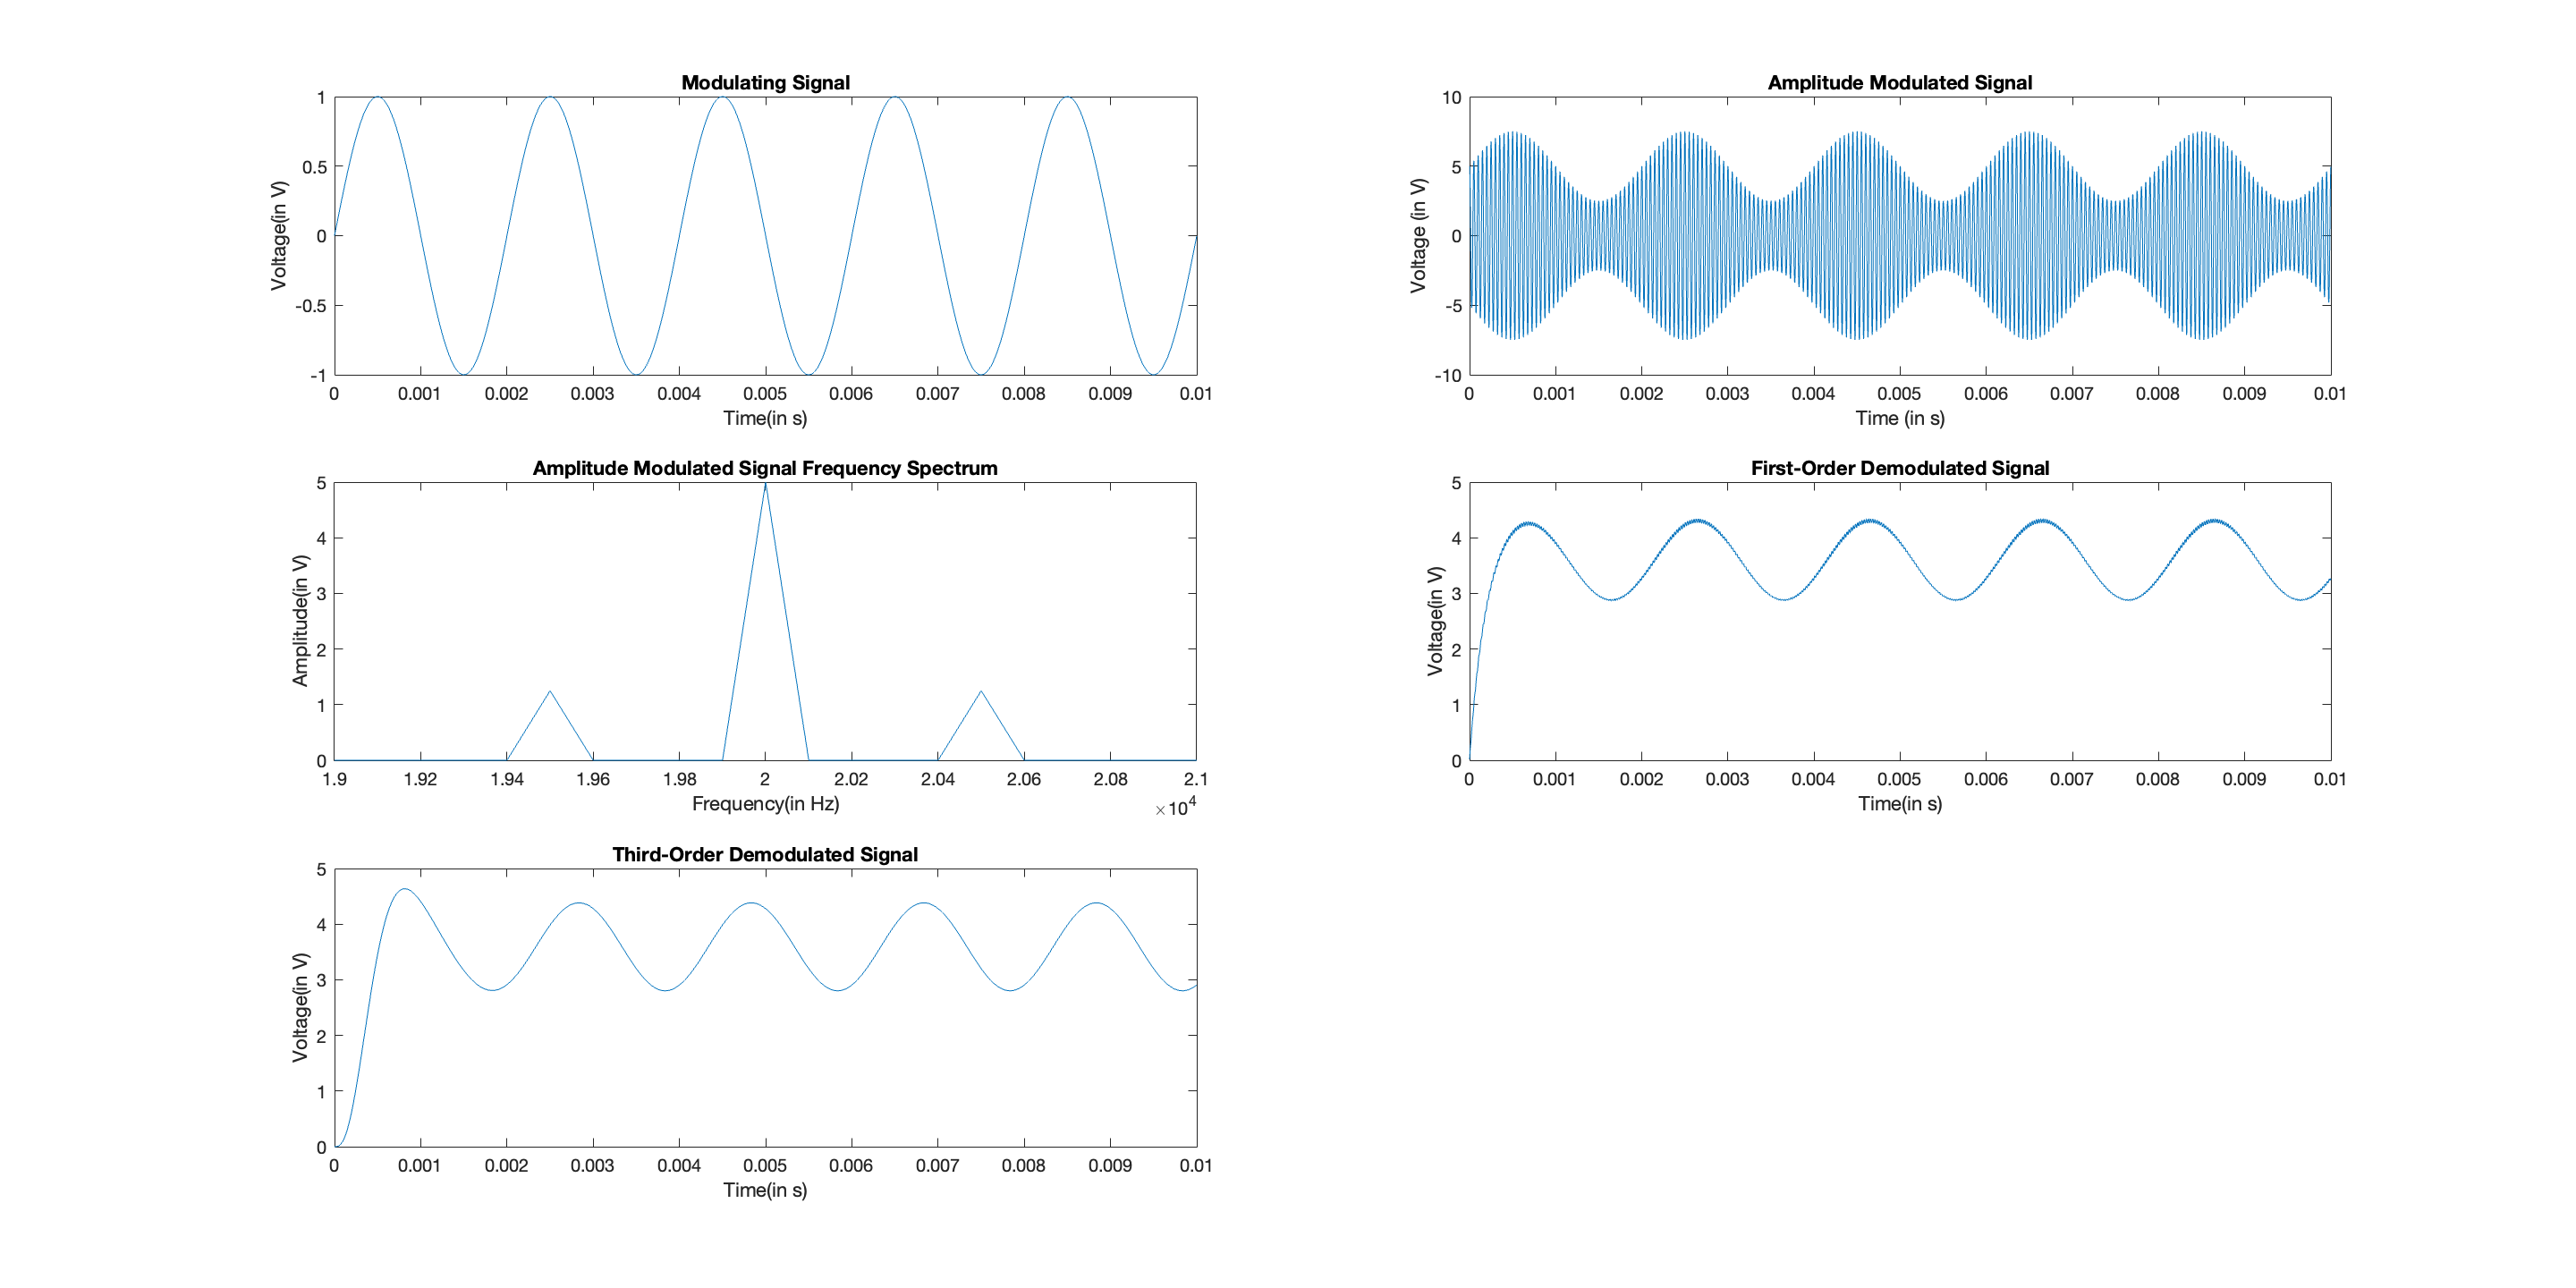
\includegraphics[width=1\textwidth]{images/prelab_problem2.png}
    \caption{AM Demodulator}
    \label{fig:AM_Demodulator}
\end{figure}

\begin{figure}[H]
    \centering
    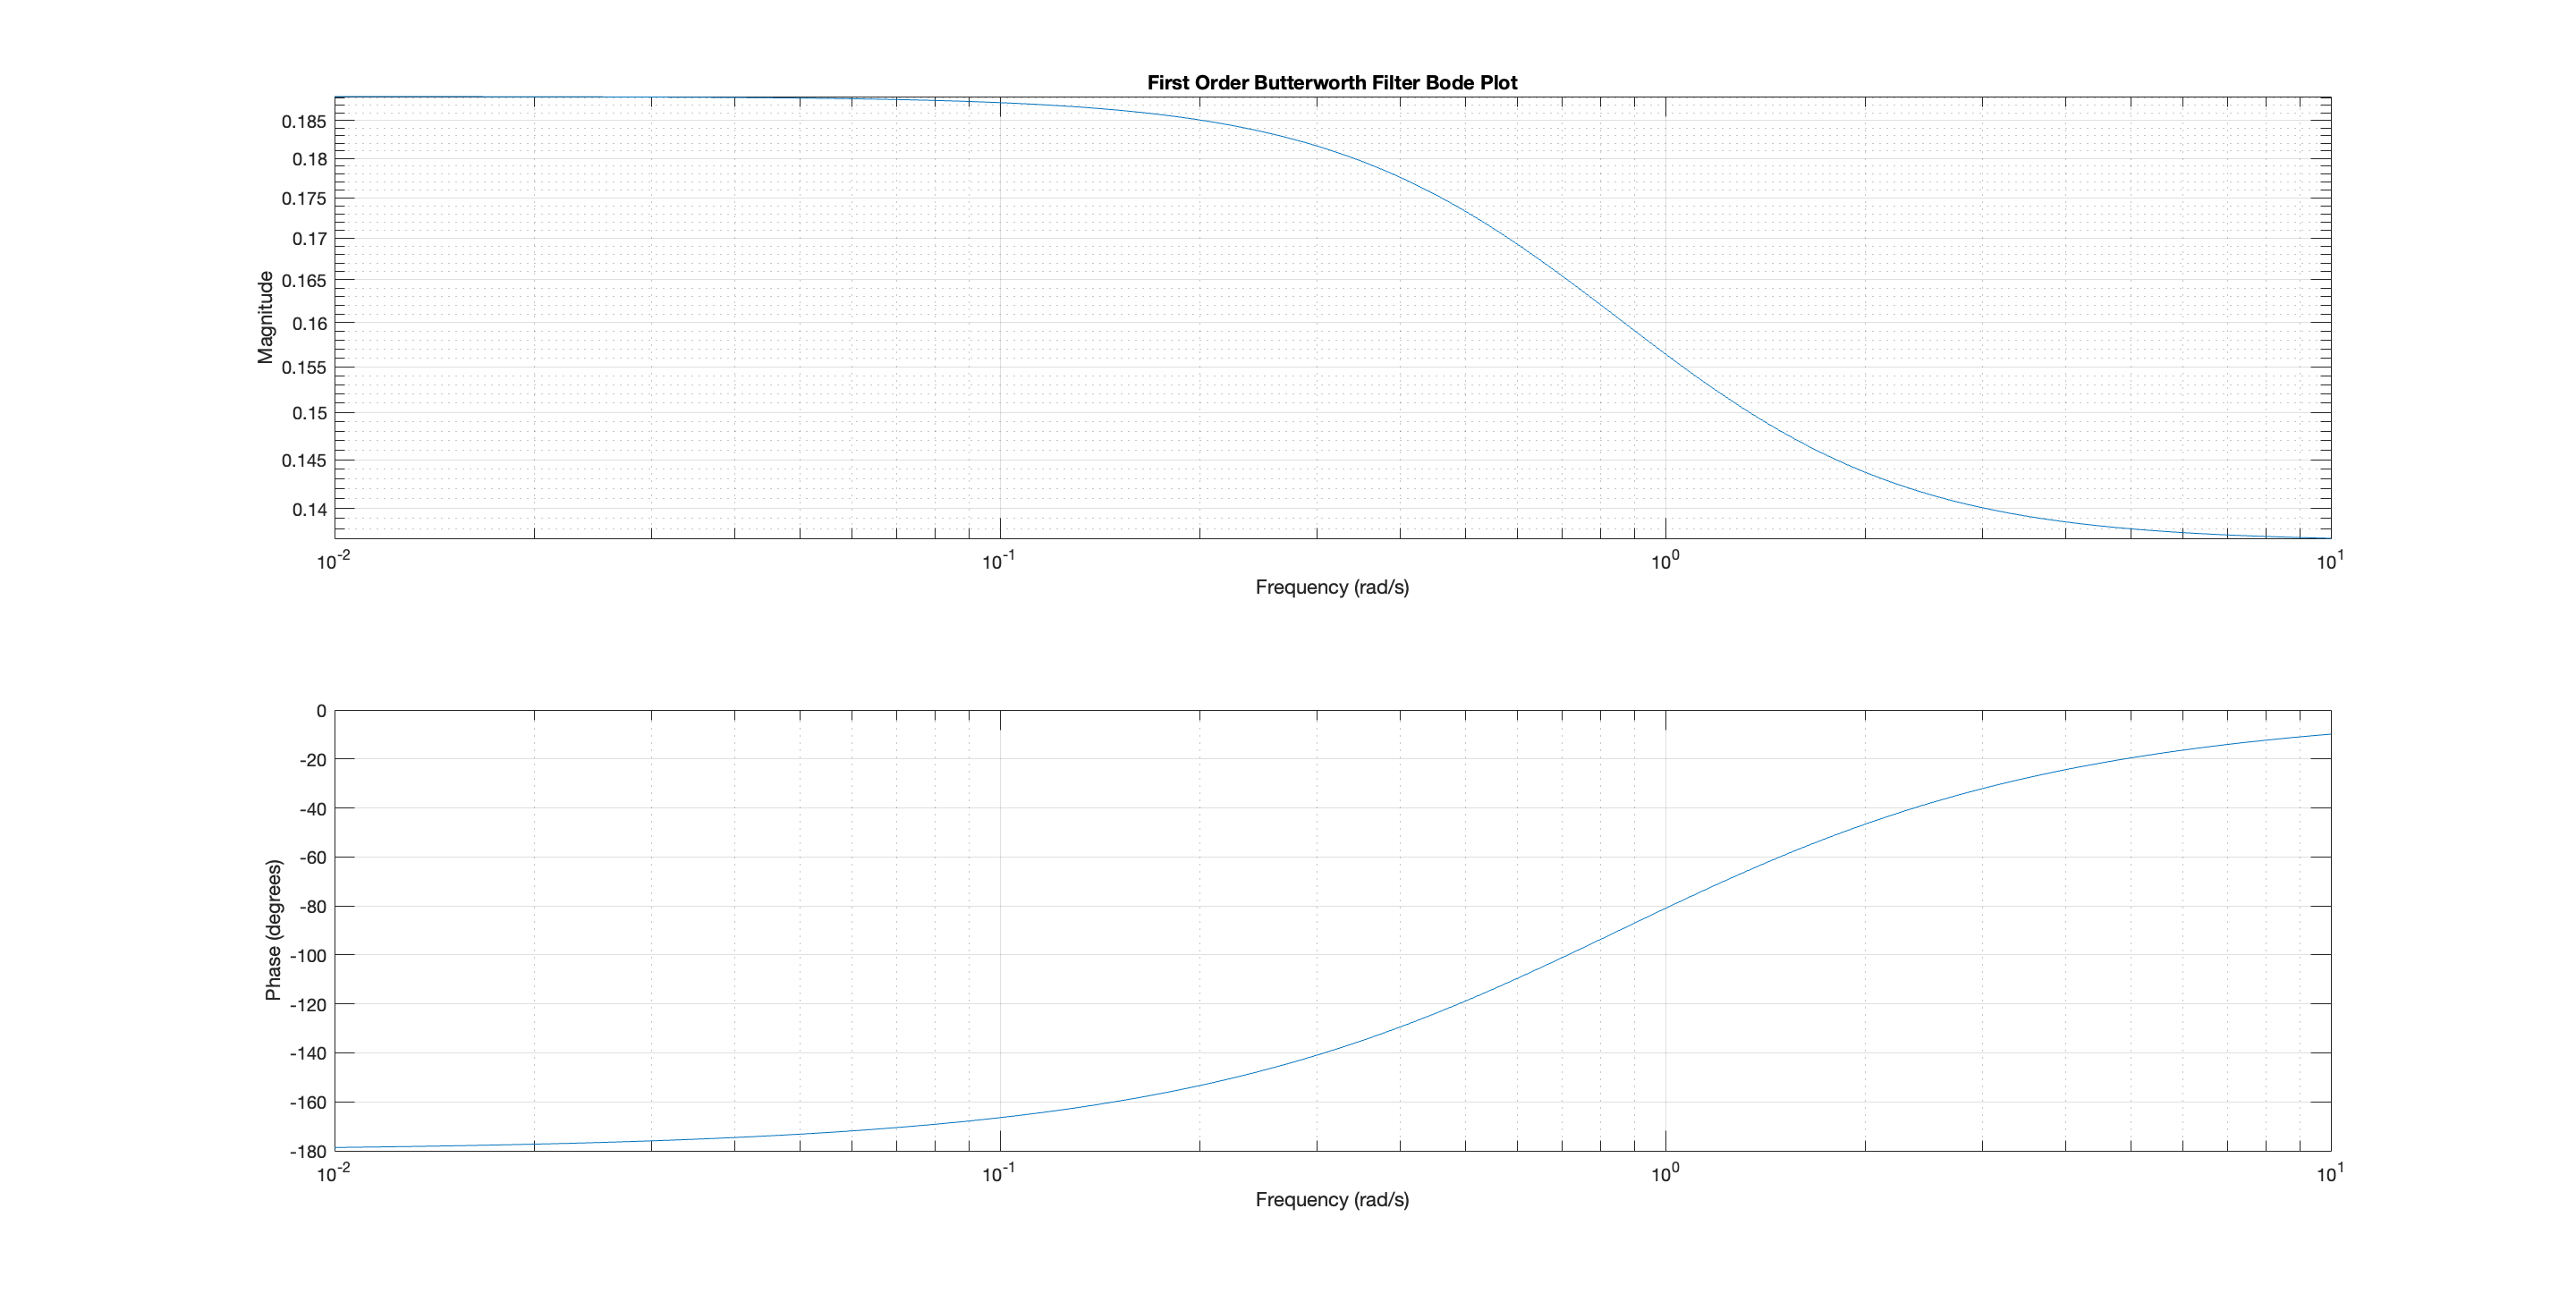
\includegraphics[width=1\textwidth]{images/prelab_problem2_firstorder.png}
    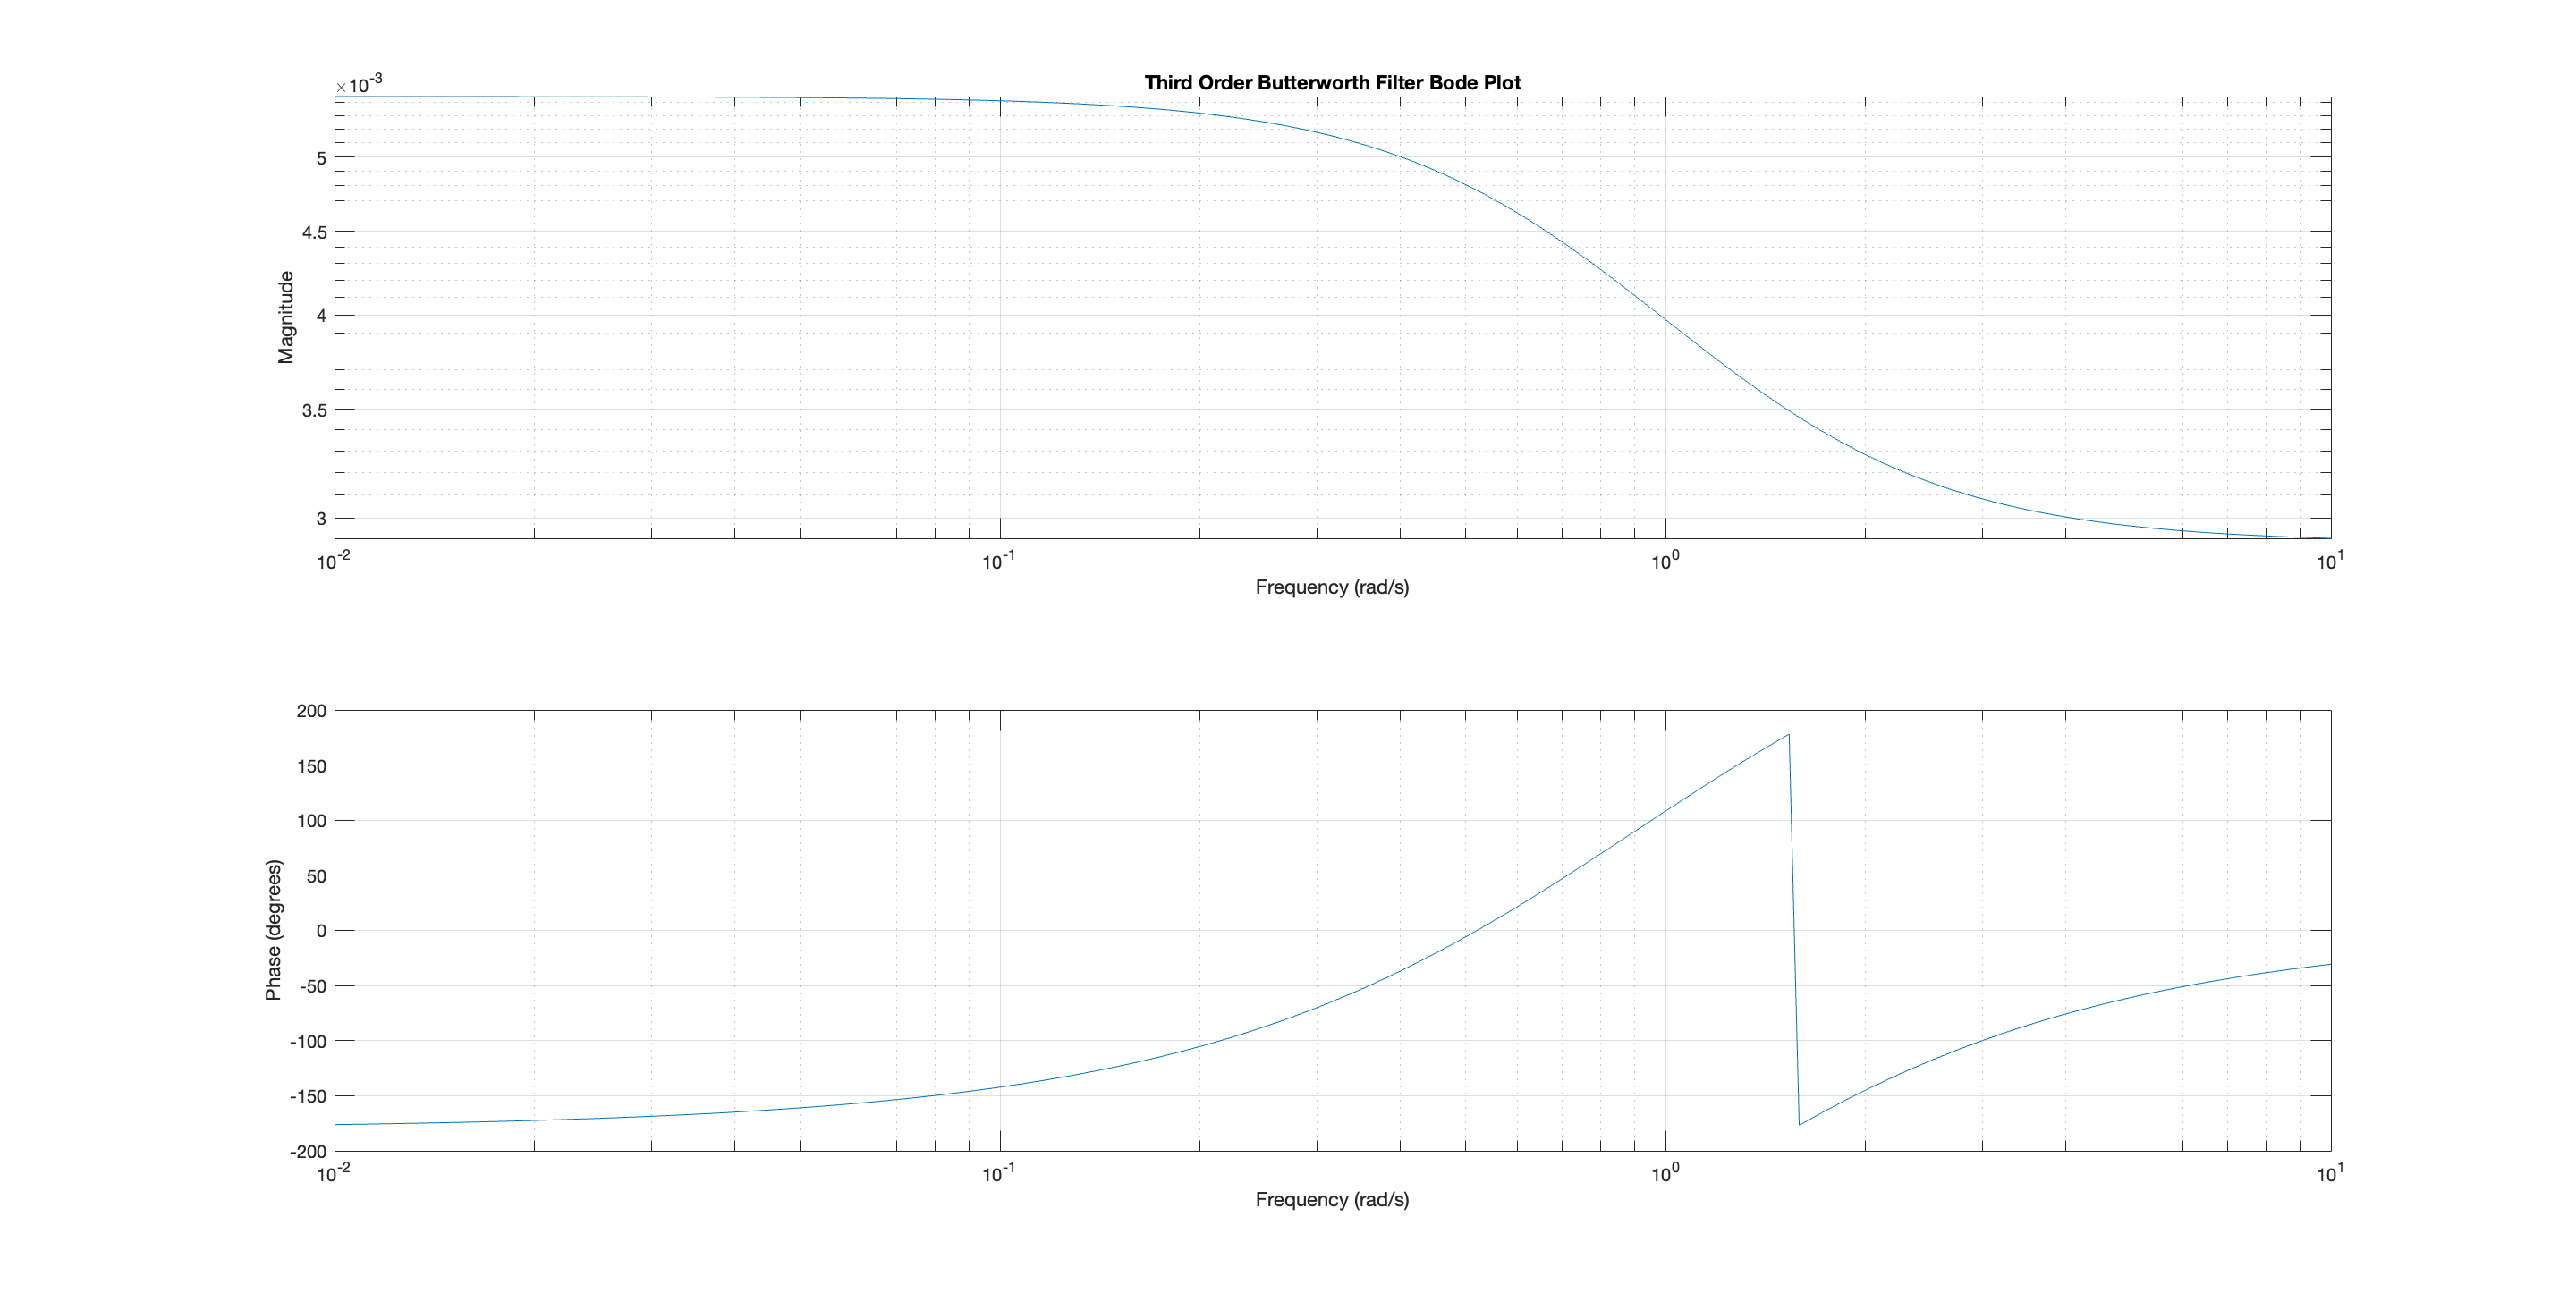
\includegraphics[width=1\textwidth]{images/prelab_problem2_thirdorder.png}
    \caption{Bode plots of the butterworth filters}
    \label{fig:bode_plots}
\end{figure}

The code to plot these signals and the butterworth filters is shown in the appendix.

The higher the order of the filter, the better the de-modulated signal will be. However, the higher the order of the filter, the more expensive it will be to implement. Therefore, the order of the filter must be chosen carefully.